%        File: report.tex
%     Created: Fri Mar 27 08:00 AM 2015 G
% Last Change: Fri Mar 27 08:00 AM 2015 G

   
% \documentclass[a4paper]{article}

%%% Start of User defined preamble:

\documentclass[a4paper, 11pt]{article}
\usepackage[english]{babel}
\usepackage[T1]{fontenc} % For å bruke æøå
\usepackage[utf8]{inputenc}
\usepackage{amsmath}
\usepackage{amssymb}
\usepackage{graphicx}
\usepackage{hyperref}
\usepackage{cite}
\usepackage{changepage}
\usepackage{listings}
\usepackage[toc,page]{appendix}

\setlength{\parskip}{1em}
\setlength{\parindent}{0pt}

\lstset{
    basicstyle=\scriptsize,
    frame=single,
    keepspaces=true,
    showstringspaces=false,
    numbers=left,
    breaklines=true
}

\title{Monte Carlo Simulations \\
Report: Problem Sheet 5 \\ A real-world application of MCMC}
\author{Kristian Bjørke}
\date{09.04.2015}

%%% End of User defined preamble:

\bibliographystyle{abbrv}

\begin{document}
\maketitle

\begin{abstract}
  In this project we have used a Markov Chain Monte Carlo(MCMC) method to
  decrypt a substitution cipher message, using statistical properties 
  of the english language. By obtaining these statistical properties 
  from analysing ``War and Peace'' by Lev Tolstoy and using a MCMC 
  computer program written in R we have  decoded a message starting with 
  ``DK PDUJVDO KSOSIUXAP DIUK  KAOSOQ BQ UMS HVSKSVCDUXAP AR$\dots$''. 
  We found the decoded message to be a paragraph taken from ``On the 
  Origin of Species'' by Charles Darwin starting with ``AS NATURAL 
  SELECTION ACTS SOLELY BY THE PRESERVATION OF$\dots$''.
\end{abstract}

\newpage
\tableofcontents
\newpage

\section{Introduction}

The purpose of this project is to use a Markov Chain Monte Carlo(MCMC) 
process to decrypt a encrypted text. We will focus on text that has been 
encrypted by the substitution cipher, which means that each letter in 
the alphabet has been replaced by another letter in the alphabet.

Each student have been given such a encrypted substitution cipher text.
Following is the one that I was given:

\begin{adjustwidth}{1.5em}{0pt}
  \small
  DK PDUJVDO KSOSIUXAP DIUK KAOSOQ BQ UMS HVSKSVCDUXAP AR
  HVARXUDBOS ZANXRXIDUXAPK, SDIM PSF RAVZ FXOO USPN XP D RJOOQ-KUAITSN 
  IAJPUVQ UA UDTS UMS HODIS AR, DPN RXPDOOQ UA SEUSVZXPDUS, XUK
  AFP OSKK XZHVACSN HDVSPU-RAVZ DPN AUMSV OSKK-RDCAJVSN RAVZK FXUM
  FMXIM XU IAZSK XPUA IAZHSUXUXAP.
\end{adjustwidth}

The papers \cite{Diaconis}, \cite{Chen} and \cite{Kocmanek} have been helpfull
while creating the R program for the Markov Chain Monte Carlo process of
decoding. While \cite{Landgraf} was helpfull to make a program that could
aquire the nececary statistics about english text needed for the decryption.

First we will outline the Markov Chain Monte Carlo decryption method that
we will use to decrypt the substitution cipher text. Then we will decribe how
we will obtain the nececary statistics about english texts by analysing the
text ``War and Peace'' by Lev Tolstoy.

After this we will present some results from applying the MCMC method to
our given text and a example text, and discuss the quality of the results.
Last we will finish with a conclusion where we sum up our findings.

At the end of the text we will include listings of the R code that was used
in this project. The source code, results and other files relevant for this
project are also available from the following GitHub repository:

\href{http://github.com/kbjorke/MCS-Problem-5}{http://github.com/kbjorke/MCS-Problem-5}

\section{Markov Chain Monte Carlo decryption method}

The MCMC method that I will be using i based mainly on \cite{Kocmanek}.

We will view the substitution ciphering as applying a function $g$ on the
message, which we call the plaintext. This function maps the text from the
decoded space into the encrypted space by returning a replacement character
for each character.

We are given an encrypted text, called the ciphertext, which has been 
encrypted by a unknown cipher function $g$, and we want to find the 
inverse function $f = g^{-1}$ that maps the ciphertext back to the plaintext,
which contains the decoded message.

We assume that the encrypted text we are given is based on a plaintext 
written in english. Characteristic for english texts are the transition 
probability matrix $M(X,Y)$ and the character probabilities $p(X)$, where
$X$ and $Y$ are any characters.

The probability matrix $M(X,Y)$ gives us the probability that the character
$Y$ will follow the character $X$ in an arbitrary english text. The
character probabilites $p(X)$ gives the probability of $X$ beein a randomly
selected character in an english text. A better way is to call $p(X)$ the
relative frequency of the character $X$ appearing in an english text.

We will attempt to find the decryption key $f$ by solving it as a maximum
likelihood problem. For this purpose we define the score function $\pi(f)$ 
for a given key $f$:

\begin{equation}
  \pi(f) = \lambda_1 \sum_{i=1}^{N} p(f(s_i)) + 
  \lambda_2 \sum_{i=1}^{N-1} M(f(s_i),f(s_{i+1}))
  \label{eq:ScoreFunc}
\end{equation}

, where $s_1,s_2,\dots,s_N$ are the consecutive characters in the ciphertext
and $N$ is the length of the ciphertext. The parameters $\lambda_1$ and 
$\lambda_2$ are weights that determine if we want to emphasize the
transition probabilities or the character probabilities. We have the conditions
$\lambda_1 + \lambda_2 = 1$ and $\lambda_1, \lambda_2 \geq 0$.

We will use a Markov Chain Monte Carlo process to find the decryption key
$f$ that maximize the score function $\pi(f)$.

To choose an initial decryption key to start the Markov Chain I suggest to
find the relative frequencies of the characters in the ciphertext, compare 
these with the relative frequencies in english texts. Then assign the most
frequent character in the ciphertext to the most frequent in english texts, 
the second most frequent with the second most frequent and so on, untill
we have an initial decryption key.

Then start the Markov Chain by repeating the following steps, and denote
$t$ as the iteration number:

\begin{enumerate}
  \item Create a new key $f_{t+1}$, where we only swap two characters of 
  the current key $f_t$.

  \item Calculate the acceptance ratio $a_t$ defined as
  \[
    a_t = \left( \frac{\pi(f_{t+1})}{f_{t}} \right)^p
  \]
  , where $p$ is the scaling parameter.

  \item Draw a random uniform distributed number $u_t$ in the range [0,1].

  \item If the acceptance ratio is larger then the random number, 
  $a_t \geq u_t$, we accept the new key and discard the current key, 
  otherwise we reject the new key and keep the current key.
\end{enumerate}

The scaling parameter $p$ is used to adjust the acceptance ratio, so that
we can avoid a local maximum or avoid to much variations around a maximum.

\section{English language properties}

In order to use the MCMC decryption methods we need to find the transition
probability matrix $M(X,Y)$ and the character probabilities $p(X)$ for
english texts. In \cite{Landgraf} there is presented a way to obtain this by
analysing a sufficiently long english text. The length of the text is
important, because it make it statistically representative for a general
english text. 

The text we will use for this analysis is the english translation of 
"War and Peace" by Lev Tolstoy, which contains about 3.1 million characters. 
This is the same text as used in \cite{Landgraf}. The text can be downloaded
from Project Gutenberg in .txt format 
\footnote{\href{http://www.gutenberg.org/ebooks/2600}
{http://www.gutenberg.org/ebooks/2600}}, which is convenient for the analysis.

The analysis was done by first formating the text so that only letters from
the english alphabeth A-Z and whitespaces remained. Non-english letters was
replaces by corresponding english letters. All other symbols was replaces by
whitespaces.

Then we used a R script to loop through all the characters of the text
and store the frequency of each characters `` '', ``A'', ``B'', 
$\dots$, ``Z'' and also the frequency of the ordered pair of two 
characters ``XY''. At the end we normalized each row of the matrix $M(X,Y)$
and the function $p(X)$ to 1.

\begin{figure}[h!]
  \centering
  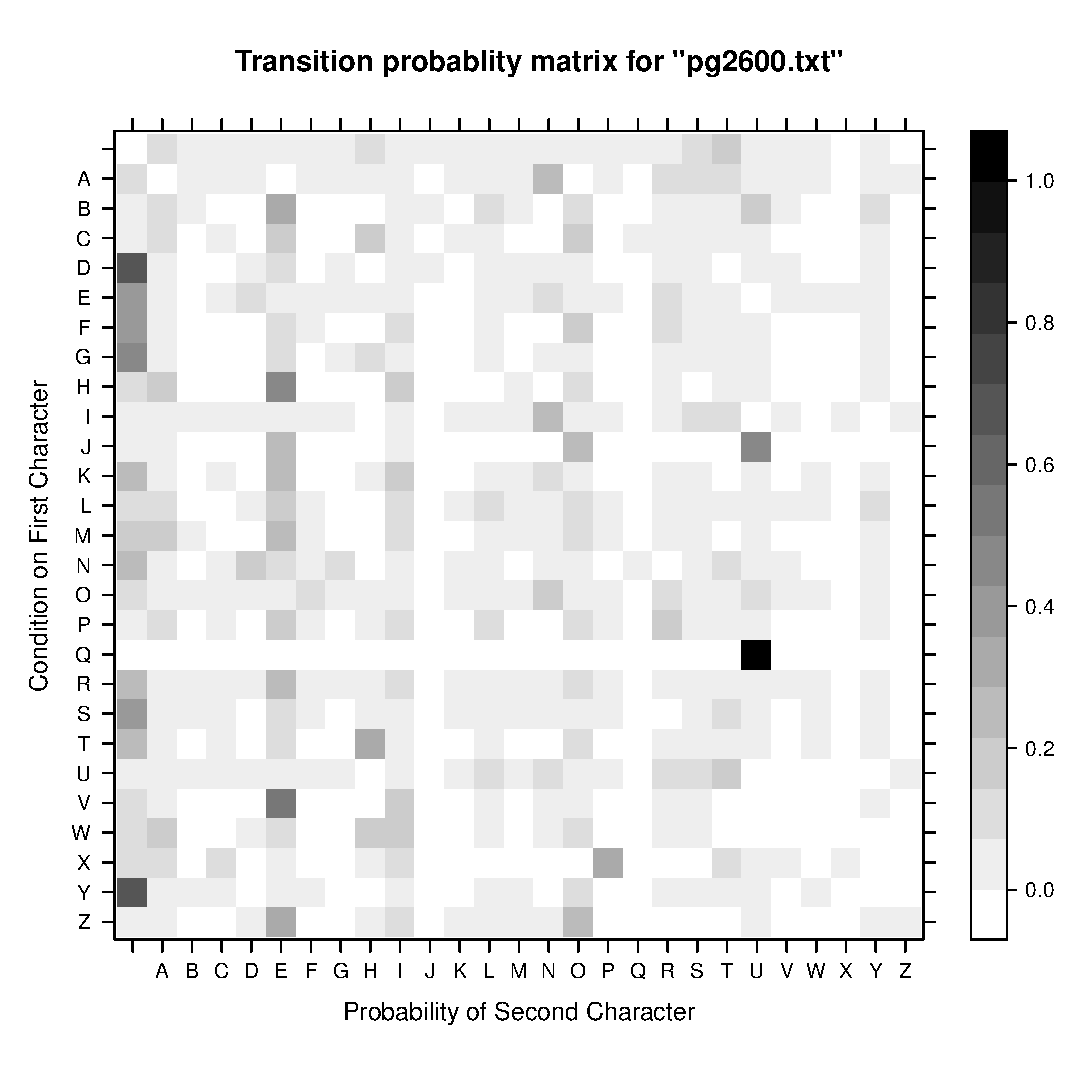
\includegraphics[width=0.7\textwidth]{transprob_matrix-pg2600-.eps}
  \caption{Transition probability matrix $M(X,Y)$ based on the text
    ``War and Peace'' by Lev Tolstoy. For comparison see \cite{Landgraf}.}
  \label{fig:TransProbMat}
\end{figure}

\begin{figure}[h!]
  \centering
  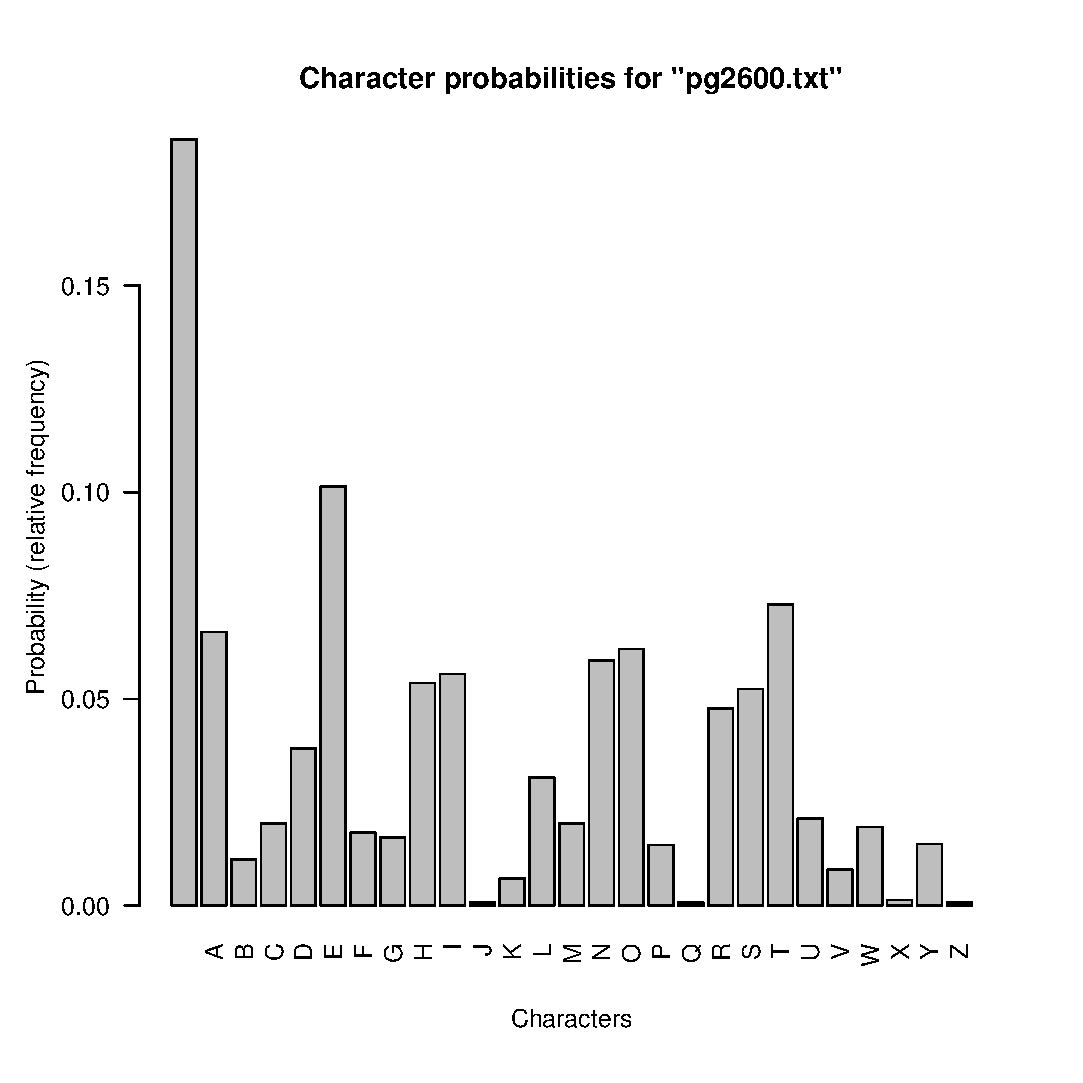
\includegraphics[width=0.7\textwidth]{char_prob-pg2600-.eps}
  \caption{Character probabilities $p(X)$ based on the text
  ``War and Peace'' by Lev Tolstoy. For comparison see 
  \href{http://en.wikipedia.org/wiki/Letter_frequency}{http://en.wikipedia.org/wiki/Letter\_frequency}}
  \label{fig:CharProb}
\end{figure}

The result from this analysis of ``War and Peace'' by Lev Tolstoy can be
seen in Figure \ref{fig:TransProbMat} and Figure \ref{fig:CharProb}. From
these figures we can see some interesting feutures of english texts. First
we can see from Figure \ref{fig:TransProbMat} that the letter ``Q'' is almost
allways followed by the letter ``U''. That ``D'' and ``Y'' are the most common
letters to end a word (follow white space `` ''), etc. From Figure 
\ref{fig:CharProb} we can see that ``E'' is the most common letter in english
texts, followed by ``T''. The letters ``J'', ``Q'', ``X'' and ``Z'' are the
letters that are the least frequent in english texts.

\section{Results and discussion}

\subsection{Test case}

As a test case I have tried first to decrypt the example text given in the
Problem sheet:

\begin{adjustwidth}{2.5em}{0pt}
  \small
  MU XCA ZNFH IGNCACKU UO ANN UEN LOJUOF XMUE EMA IFNUUH
  HOWKB XMDN. EN ECL C DCUENFGH, SNKMBKCKU XCH OD AEOXMKB
  EMA DOKLKNAA DOF ENF, XEMJE ANNQNL MK MUANGD UO NPIFNAA 
  C BOOL QCK. M ODUNK ACX UENQ XCGTMKB MK UEN BCFLNK
  XENFN UEN INCJENA XNFN, CKL M AOQNUMQNA ECL C KNCFNF
  OSANFZCUMOK OD UENQ MK UEN AUWLH OF UEN ICFGOWF. AEN
  CIINCFNL UO QN UO UCTN BFNCU JCFN OD UEN LOJUOF, CKL UO
  GMTN EMQ ZNFH QWJE, UEOWBE M KNZNF UEOWBEU ENF ZMUCGGH
  MKUNFNAUNL MK UEN LMJUMOKCFH: AOQN JWQSFOWA DFCBQNKUA
  OD XEMJE XOFT UEN LOJUOF CGXCHA JCFFMNL MK EMA IOJTNUA,
  CKL MK UEN GMKMKB OD EMA ECU, CKL BNKNFCGGH ANNQNL UO
  SN NPIOWKLMKB UO ENF CA UENH XCGTNL CSOWU.
\end{adjustwidth}

Using the Markov Chain Monte Carlo decryption method described above I found 
that the encrypted text becomes:

\begin{adjustwidth}{2.5em}{0pt}
  \small
  IT WAS VERY PLEASANT TO SEE THE DOCTOR WITH HIS PRETTY
  YOUNG WIFE. HE HAD A FATHERLY, BENIGNANT WAY OF SHOWING
  HIS FONDNESS FOR HER, WHICH SEEMED IN ITSELF TO EXPRESS 
  A GOOD MAN. I OFTEN SAW THEM WALKING IN THE GARDEN
  WHERE THE PEACHES WERE, AND I SOMETIMES HAD A NEARER
  OBSERVATION OF THEM IN THE STUDY OR THE PARLOUR. SHE
  APPEARED TO ME TO TAKE GREAT CARE OF THE DOCTOR, AND TO
  LIKE HIM VERY MUCH, THOUGH I NEVER THOUGHT HER VITALLY
  INTERESTED IN THE DICTIONARY: SOME CUMBROUS FRAGMENTS
  OF WHICH WORK THE DOCTOR ALWAYS CARRIED IN HIS POCKETS,
  AND IN THE LINING OF HIS HAT, AND GENERALLY SEEMED TO
  BE EXPOUNDING TO HER AS THEY WALKED ABOUT.
\end{adjustwidth}

, with the following decryption key

\begin{table}[h]
  \centering
  \caption{Decryption key to decipher the example text given in the
  Problem sheet.}
  \begin{tabular}{l l l l l}
\{ \ \} =    &  \{F\} = R  &  \{L\} = D  &  \{R\} = J  &  \{X\} = W  \\
\{A\} = S  &  \{G\} = L  &  \{M\} = I  &  \{S\} = B  &  \{Y\} = Z  \\
\{B\} = G  &  \{H\} = Y  &  \{N\} = E  &  \{T\} = K  &  \{Z\} = V  \\
\{C\} = A  &  \{I\} = P  &  \{O\} = O  &  \{U\} = T  &  \ \\
\{D\} = F  &  \{J\} = C  &  \{P\} = X  &  \{V\} = Q  &  \ \\
\{E\} = H  &  \{K\} = N  &  \{Q\} = M  &  \{W\} = U  &  \ \\
  \end{tabular}
  \label{tab:ExampleKey}
\end{table}

The first thing that I noticed while trying to decrypt this text was that I
required a relativly large value for the scaling parameter to get good results
from the decryption. A scaling parameter of $p = 3000$ is what I found to
be the best to use to decrypt the text. But for scaling parameters larger then
500 we usually get a solution that makes sense.

When considering the weights for the score function (\ref{eq:ScoreFunc}), I 
found that I got the best results using $\lambda_1 = 0.1$ and 
$\lambda_2 = 0.9$. This means that in the decryption I have put more emphasis 
on the character probabilities $p(X)$ then the transition probabilities 
$M(X,Y)$.

Trying different values for the weights $\lambda_1$ and $\lambda_2$,
with $p = 3000$, I learned that I would get something
close to the correct key either by emphsising the character probabilities
($\lambda_1 > 0.6$) or emphasising the transition probabilities 
($\lambda_2 > 0.6$). The case of $\lambda_1 = \lambda_2 = 0.5$ gave me 
poor results compared to the other values. Excluding the character
probabilities ($\lambda_1 = 0$) gave me a solution from which we could
deduce the correct key, while exluding the transition probabilities
($\lambda_2 = 0$) did not give anything close to the correct solution.

Another thing to note is that not allways will the decryption method give
the exact correct solution for the ciphertext. The reason for this is that
the method is based on finding the key which gives the highest value for 
the score function. This will not necesarily be the correct key, because 
if the text are small, like the text we are decrypting, one can not allways
assume that they will follow the statistics of english texts given by
$p(X)$ and $M(X,Y)$.

An example of this is that when I used the decryption methods with the
parameters given above the correct key $f$ has a score function of 
$\pi(f) = 55.535$. But there exists a solution, with almost the correct
key $f'$, where the score function becomes $\pi(f') = 55.540$, which is only
slightly higher than for the correct key. The difference between the keys
$f$ and $f'$ is that in $f'$ we have \{T\} = V and \{Z\} = K as opposed to
the correct key $f$ described above.

Running the script for large Monte Carlo samples $N$ will almost allways give
the key $f'$ as a results, which I experienced while solving. But when 
presented with the key $f'$ is it easy to reason what the correct key
is supposed to be. One trial I used $N = 2000$ I got the corret key $f$ right 
out, but this is probably because the Markov Chain never encountered the $f'$
key.

\subsection{Given ciphertext}

Before given the solution for the substitution cipher text that I was given
for this problem sheet I will repeat the text as mentioned above in the
Introduction:

\begin{adjustwidth}{1.5em}{0pt}
  \small
  DK PDUJVDO KSOSIUXAP DIUK KAOSOQ BQ UMS HVSKSVCDUXAP AR
  HVARXUDBOS ZANXRXIDUXAPK, SDIM PSF RAVZ FXOO USPN XP D RJOOQ-KUAITSN 
  IAJPUVQ UA UDTS UMS HODIS AR, DPN RXPDOOQ UA SEUSVZXPDUS, XUK
  AFP OSKK XZHVACSN HDVSPU-RAVZ DPN AUMSV OSKK-RDCAJVSN RAVZK FXUM
  FMXIM XU IAZSK XPUA IAZHSUXUXAP.
\end{adjustwidth}

Using the Markov Chain Monte Carlo decryption we solved for a number of
different values for both the scaling parameter $p$ and the weights 
$\lambda_1$ and $\lambda_2$. What we found was using the same scaling function
weights as for the example case, $\lambda_1 = 0.1$ and $\lambda_2 = 0.9$,
we got results that where possible to deduce the correct key and decryption
from. Using a scaling parameter of $p = 4000$ we got

\begin{adjustwidth}{1.5em}{0pt}
  \small
  AS NATURAL SELECTION ACTS SOLELY BY THE PRESERMATION OF
  PROFITABLE GODIFICATIONS, EACH NEW FORG WILL TEND IN A FULLY-
  STOCVED COUNTRY TO TAVE THE PLACE OF, AND FINALLY TO EXTERGINATE, ITS
  OWN LESS IGPROMED PARENT-FORG AND OTHER LESS-FAMOURED FORGS WITH
  WHICH IT COGES INTO COGPETITION.
\end{adjustwidth}

, with the following decryption key

\begin{table}[h]
  \centering
  \caption{Decryption key of the initial solution of the MCMC decryption 
  method.}
  \begin{tabular}{l l l l l}
  \{ \ \} =    &  \{F\} = W  &  \{L\} = Z  &  \{R\} = F  &  \{X\} = I  \\
  \{A\} = O  &  \{G\} = Q  &  \{M\} = H  &  \{S\} = E  &  \{Y\} = J  \\
  \{B\} = B  &  \{H\} = P  &  \{N\} = D  &  \{T\} = V  &  \{Z\} = G  \\
  \{C\} = M  &  \{I\} = C  &  \{O\} = L  &  \{U\} = T  &  \ \\
  \{D\} = A  &  \{J\} = U  &  \{P\} = N  &  \{V\} = R  &  \ \\
  \{E\} = X  &  \{K\} = S  &  \{Q\} = Y  &  \{W\} = K  &  \ \\
  \end{tabular}
  \label{tab:FirstKey}
\end{table}

We see that we here have a text that is almost decrypted, except for some 
words that does not make sense in the paragraph, like ``PRESERMATION'',
``GODIFICATIONS'', ``FULLY-STOCVED'' and others. But we can deduce some changes
to these word so that they make more snese. These are changing 
\{C\} = V, \{Z\} = M, \{T\} = K. As a consequence of these changes
we also has that \{W\} = G. Applying these changes gives us the final
solution for the decrypted text as:

\begin{adjustwidth}{1.5em}{0pt}
  \small
  AS NATURAL SELECTION ACTS SOLELY BY THE PRESERVATION OF
  PROFITABLE MODIFICATIONS, EACH NEW FORM WILL TEND IN A FULLY-STOCKED 
  COUNTRY TO TAKE THE PLACE OF, AND FINALLY TO EXTERMINATE, ITS
  OWN LESS IMPROVED PARENT-FORM AND OTHER LESS-FAVOURED FORMS WITH
  WHICH IT COMES INTO COMPETITION.
\end{adjustwidth}

, with the following decryption key

\begin{table}[h]
  \centering
  \caption{Decryption key to the final and correct solution for the 
  ciphertext given to me.}
  \begin{tabular}{l l l l l}
  \{ \ \} =    &  \{F\} = W  &  \{L\} = Z  &  \{R\} = F  &  \{X\} = I  \\
  \{A\} = O  &  \{G\} = Q  &  \{M\} = H  &  \{S\} = E  &  \{Y\} = J  \\
  \{B\} = B  &  \{H\} = P  &  \{N\} = D  &  \{T\} = K  &  \{Z\} = M  \\
  \{C\} = V  &  \{I\} = C  &  \{O\} = L  &  \{U\} = T  &  \ \\
  \{D\} = A  &  \{J\} = U  &  \{P\} = N  &  \{V\} = R  &  \ \\
  \{E\} = X  &  \{K\} = S  &  \{Q\} = Y  &  \{W\} = G  &  \ \\
  \end{tabular}
  \label{tab:FinalKey}
\end{table}

One thing need to be noted about this solution decryption key. That is that 
there are some characters in the code that are not used in the ciphertext.
These are less frequent letter Q, Z, J, see Figure \ref{fig:CharProb}, and G.
If we shuffle these around in the decryption key we would get the same 
solution for the decrypted text. So the correct decryption for the cipher 
letters \{G\}, \{L\}, \{Y\} and \{W\} are still unknown. With this in 
consideration we can find the encryption key $g$ used to cipher the text by
inverting the decryption key $f$, this gives:

\begin{table}[h]
  \centering
  \caption{Encryption key used to create the ciphertext given to me.
  Key for Q, Z, J and G are suggestions, since they are not present in the
  text.}
  \begin{tabular}{l l l l l}
  \ \ \ = \{ \ \}  &  F = \{R\}  &  L = \{O\}  &  R = \{V\}  &  X = \{E\} \\
  A = \{D\}  &  G = \{W\}  &  M = \{Z\}  &  S = \{K\}  &  Y = \{Q\}  \\
  B = \{B\}  &  H = \{M\}  &  N = \{P\}  &  T = \{U\}  &  Z = \{L\}  \\
  C = \{I\}  &  I = \{X\}  &  O = \{A\}  &  U = \{J\}  &  \ \\
  D = \{N\}  &  J = \{Y\}  &  P = \{H\}  &  V = \{C\}  &  \ \\
  E = \{S\}  &  K = \{T\}  &  Q = \{G\}  &  W = \{F\}  &  \ \\
  \end{tabular}
  \label{tab:CipherKey}
\end{table}


\section{Conclusion}

We have now shown how we can use Markov Chain Monte Carlo method to
decrypt substitution cipher texts. This method has been based on the analysis
of a long english text, ``War and Peace'' by Lev Tolstoy, where we have
calculated the character probabilities and transition probabilities 
characteristic for english texts.

Using the MCMC method described above, with a scaling parameter of $p = 4000$
and score function weights of $\lambda_1 = 0.1$ and $\lambda_2 = 0.9$, we found
a solution that was almost correct. After some small changes by deduction we
found that the ciphertext that started with ``DK PDUJVDO KSOSIUXAP DIUK  
KAOSOQ BQ UMS HVSKSVCDUXAP AR$\dots$'', in decrypted form appeared as
``AS NATURAL SELECTION ACTS SOLELY BY THE PRESERVATION OF$\dots$''.

I have found that the solution of the encrypted text mirrors a sentence 
taken from Chapter 6 of the book ``Of the Origin of Species'' By Charles Darwin,
see Figure \ref{fig:Darwin}.

A interesting thing that could be done is to find the ideal value for 
$\lambda_1$ and $\lambda_2$. This can be done in the analysis of the 
reference text as suggested by \cite{Kocmanek}. Otherwise it could be done 
by trying to solve for diffrent values of $\lambda_1$ and $\lambda_2$ and see
when we get the closes result to the correct solution.

Another interessting thing could be to also try to add the three characters
probabilities $T(X,Y,Z)$ in or analysis of english texts and as a third part of
our score function, introducing a new weight parameter $\lambda_3$.

And combining the two suggestions above we could try to see if we could 
solve the decryption directly to the correct solution without having to 
deduce one or more of the characters in the code key as we did.

\begin{figure}[h!]
  \centering
  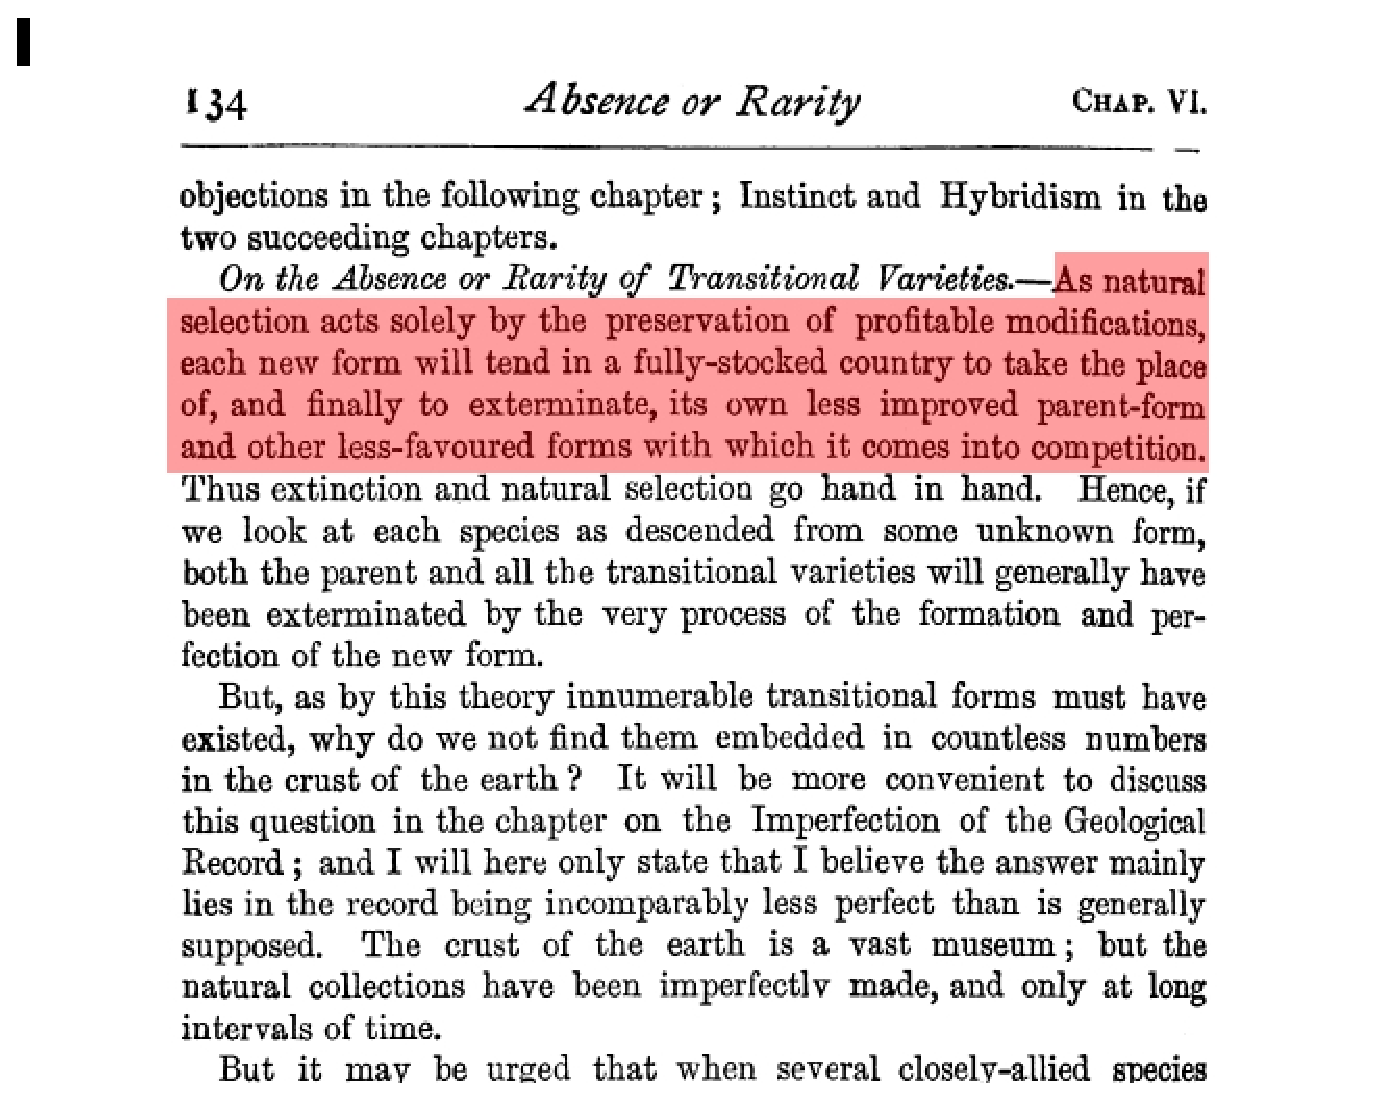
\includegraphics[width=1.0\textwidth]{decrypted_text_source_Darwin_OriginOfSpieces.eps}
  \caption{Page from ``Of the Origin of Species'' by Charles Darwin where I
  have identified the source of the encrypted text I have been given.}
  \label{fig:Darwin}
\end{figure}

\bibliography{references}

\newpage

\begin{appendix}

  {\huge{\bf Appendix}}
  
  \section{Decryption output for the example text}
 
  \verb+output_04-01_13-32.txt+
  \lstinputlisting[language=r]
  {../output-example_encrypted_text/output_04-01_13-32.txt}

  \section{Decryption output for the given ciphertext}
  
  \section{Code Listings}
\end{appendix}



\end{document}


